\input{praeambel_gesina}

\usepackage{pgf,tikz}
\usetikzlibrary{arrows}

\begin{document}

	%Abbildung 3.1
		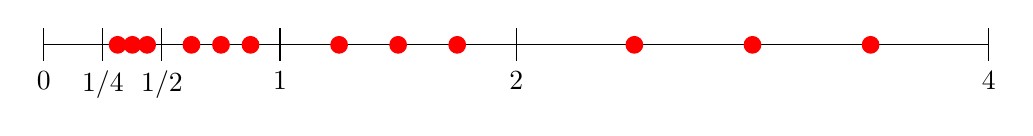
\begin{tikzpicture}[scale=3]
		    \draw(0,0)--(4,0);
		%Vertikale Striche
		    \foreach \x/\xtext in {0/0,0.25/{1/4},0.5/{1/2},1/1,2/2,4/4}
		      \draw(\x,2pt)--(\x,-2pt) node[below] {\xtext};
		%Rote Kreise zeichnen
		      \foreach \x in {0.3125,0.375,0.4375,0.625,0.75,0.875,1.25,1.5,1.75,2.5,3,3.5}
		      	\draw[fill,red] (\x,0) circle (1pt);
		  \end{tikzpicture}



%Abbildung 3.2
\centering
	\begin{tikzpicture}[scale=3]
		    \draw(0,0)--(3,0);
		    \Large
		%Vertikale Striche
		    \foreach \x/\xtext in {1/{$x$},2/{$\tilde{x}$}}
		      \draw(\x,2pt)--(\x,-2pt) node[below] {\xtext};
		    \foreach \x/\xtext in {0.5/[,1.48/),1.5/[}
		    	\node at (\x,0) {\bfseries \xtext};
		    \node at (1,0.2) {$E(x)$};
	\end{tikzpicture}
	
%Abbildung 3.4
	\begin{minipage}{0.48\linewidth}
	\centering
	\begin{tikzpicture}[line cap=round,line join=round,>=triangle 45,x=1.0cm,y=1.0cm]
	\draw[->,color=black] (0,0) -- (6,0);
	\draw[->,color=black] (0,0) -- (0,4.5);
	\clip(-1,-0.6) rectangle (6,6.5);
	\draw[smooth,samples=100,domain=0.5:5.5] plot(\x,{1/10*((\x)-3)^3+2});
	\draw [dash pattern=on 3pt off 3pt] (1.1,1.31)-- (1.1,0);
	\draw [dash pattern=on 3pt off 3pt] (0,1.31)-- (1.1,1.31);
	\draw [dash pattern=on 3pt off 3pt] (0,2.8)-- (5,2.8);
	\draw [dash pattern=on 3pt off 3pt] (5,2.8)-- (5,0);
	\draw (2.86,0) node[anchor=north west] {$x$};
	\draw (-0.6,2.18) node[anchor=north west] {$y$};
	\draw [color=black] (3,2)-- ++(-2pt,-2pt) -- ++(4pt,4pt) ++(-4pt,0) -- ++(4pt,-4pt);
	\fill  (0,2) circle (1.5pt);
	\fill  (3,0) circle (1.5pt);
	\end{tikzpicture}
	Schlechte Kondition
	\end{minipage}\hfill
	\begin{minipage}{0.48\linewidth}
	\centering 
	\begin{tikzpicture}[line cap=round,line join=round,>=triangle 45,x=1.0cm,y=1.0cm]
	\draw[->,color=black] (0,0) -- (6,0);
	\draw[->,color=black] (0,0) -- (0,4.5);
	\clip(-1,-0.6) rectangle (6,6.5);
	\draw[smooth,samples=100,domain=1.0:5.0] plot(\x,{1/100*((\x)+2)^3+0.5});
	\draw [dash pattern=on 3pt off 3pt] (2.66,1.51)-- (2.66,0);
	\draw [dash pattern=on 3pt off 3pt] (4,0)-- (4,2.66);
	\draw [dash pattern=on 3pt off 3pt] (4,2.66)-- (0,2.66);
	\draw [dash pattern=on 3pt off 3pt] (0,1.51)-- (2.66,1.51);
	\draw (3.26,0) node[anchor=north west] {$x$};
	\draw (-0.6,2.38) node[anchor=north west] {$y$};
	\fill  (0,2.16) circle (1.5pt);
	\fill  (3.5,0) circle (1.5pt);	
	\draw [color=black] (3.5,2.16)-- ++(-2pt,-2pt) -- ++(4pt,4pt) ++(-4pt,0) -- ++(4pt,-4pt);
	\end{tikzpicture}
	Gute Kondition
	\end{minipage}	

%Abbildung 3.5
	\begin{tikzpicture}[>=triangle 45]
		\draw (0,-2.2) -- (0,2.1);
		\draw[->] (0,0) -- (3,0);
		\draw[->] (0,0) -- (1.5,-1.5);
		\draw[->] (0,0) -- (1.5,1.5);
		\draw (2.6,1) node {$x=\tilde{x}=|\tilde{y}|\approx|y|$};
	\end{tikzpicture}
	
%Abbildung 3.6
\begin{minipage}{0.73\linewidth}
		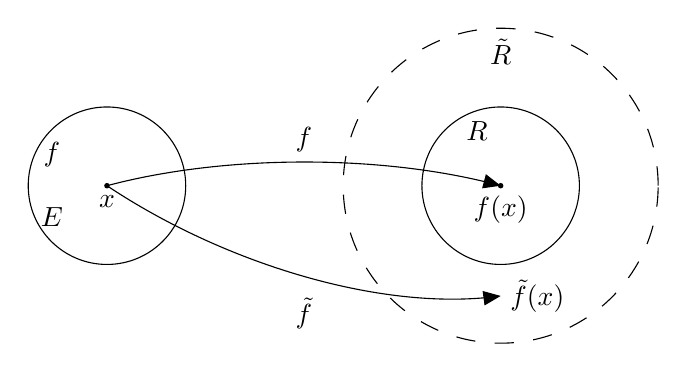
\begin{tikzpicture}[>=triangle 45]
			%Linker Kreis mit allen Objekten
				\draw (0,0) circle (1);
				\draw (-0.7,0.4) node {$f$};
				\draw (-0.7,-0.4) node {$E$};
				\fill (0,0) node[below]{$x$} circle (1pt);
			%Pfeile:
				\draw[->] (0,0) .. controls (1.5,0.4) and (3.5,0.4).. (5,0);
				\draw[->] (0,0) .. controls (1.5,-1)  and (3.5,-1.6)..(5,-1.4) node[right] {$\tilde{f}(x)$};
				\draw (2.5,0.3) node[above] {$f$};
				\draw (2.5,-1.3) node[below] {$\tilde{f}$};
				
			%Rechte Seite
				\draw (5,0) circle (1);
				\draw[dash pattern=on 7pt off 7pt] (5,0) circle (2);
				\fill (5,0) node[below]{$f(x)$} circle (1pt);
				\draw (5,1.7) node {$\tilde{R}$};
				\draw (4.7,0.7) node {$R$};
			\end{tikzpicture}
	\end{minipage}
	\begin{minipage}{0.25\linewidth}
			\begin{align*}
				R&=f(E)\qquad\text{stabil}\\
				\tilde{R} &= \tilde{f}(E)\qquad\text{instabil}\\
			\end{align*}
	\end{minipage}

%Abbildung unter Formel (4.2.4)
	\begin{tikzpicture}
		%Dreiecke zeichnen
		\foreach \x in {0,5}
		{
			\draw (\x,0) -- (\x+4,0) -- (\x,4) -- cycle;
			\draw (\x,2.5) node[left] {$k$} -- (\x+1.5,2.5);
			\draw (\x+1.5,4.5) node {$k$};
		}
		\draw[dash pattern=on 3pt off 3pt] (6.5,0) -- (6.5,4);
		\draw (5,1) node[left] {$i$} -- (8,1);
	\end{tikzpicture}
\end{document}